\documentclass[../main.tex]{subfiles}

\begin{document}

\subsection{Functional requirements}

In order to achieve the objectives listed
in \cref{sec:objectives}, the following activities 
and operations should be expected by the user 
and the \gls{uav} system:

\begin{enumerate}
    \item The users of the system are authorized
        individuals and organizations to track, monitor or survey
        some moving objects.
    \item The user should supply the 
        profile of the targets 
        and their movement details/patterns
        to us for the \gls{rl}.
    \item The user should receive 
        a \uav integrated system consisting of 
        an \anafi drone, a \textsc{r}aspberry \textsc{p}i,
        and a \gls{drl} model after the \gls{ml} training
        is complete.
    \item The system should take pictures, capture videos
        or record other physical properties using
        suitable sensors of the intended
        targets according to the needs
        of the user.
    \item The user should receive some 
        guidance and support 
        to handle the system.
    \item The user should agree on 
        the terms and conditions 
        which limit the type of usages and 
        ensure that it aligns with the legislations
        related to the use of drones in that area.
    \item The system should only allow 
        authorized users 
        to view the collected pictures and 
        data from the \anafi system.
\end{enumerate}

\Cref{fig:use-case-diagram} shows the use cases that can
happen between the system and the user. The details of their
interactions are summarized in \cref{tab:use-case-summaries}.

\begin{figure}[p] 
    \centering
    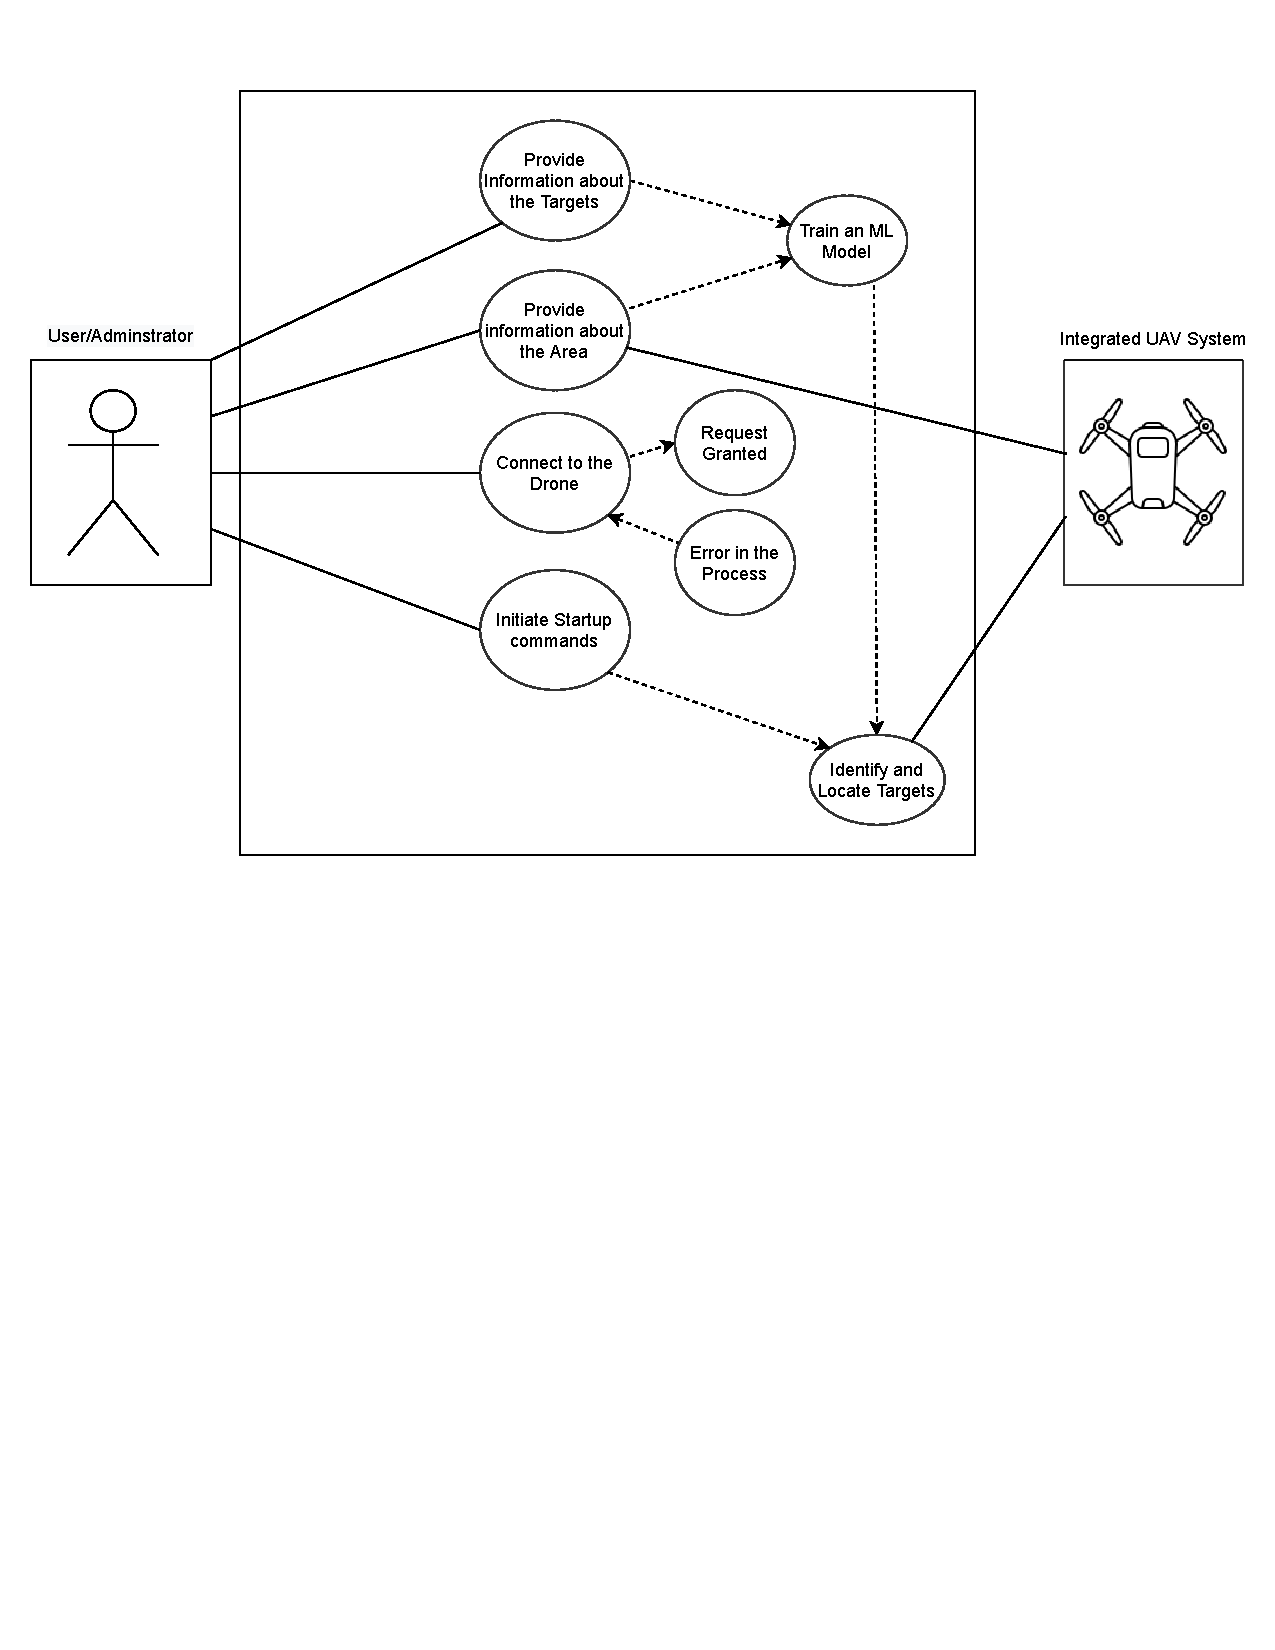
\includegraphics[width=1.0\textwidth]{use-case-diagram} 
    \caption{The use case diagram for the system proposed 
            in this project depicting possible interactions 
            between the user and the system.}
    \label{fig:use-case-diagram} 
\end{figure}

\begin{table}[p]
    \centering
    \caption{Summary of the use cases of the system.}
    \label{tab:use-case-summaries}
    \begin{tabularx}{\textwidth}{ p{3.5cm} X }
        \toprule

        \textit{Use case} & \textit{Description} 
        \\

        \midrule

        Provide information about the targets
            & The main types of information required are
            the targets' mobility pattern and their 
            appearances. 
            The former will be used in the \gls{rl} training
            for the autonomous navigation while the latter
            will be used in the \gls{ml} object detection for
            the reward in the \gls{rl} training and the
            actual mission.
        \\
        Provide information about the area
            & The types of obstacles in the area are 
            important to be known so that they can be
            simulated. The \uav will learn to ignore them
            during the training making them visit only
            the targeted objects.
        \\
        Connect to the drone
            & Only the authorized user is allowed to connect
            to the drone using the command and control system.
            If this is the case, the connection request is
            granted. Otherwise, an error will be returned.
        \\
        Initiate startup commands
            & The \uav by this point is already autonomous.
            It uses the \gls{rl} and object detection models
            trained earlier to visit the intended targets 
            in the fastest time possible. 
            The authorized user only needs to send
            a start command to the \uav, and it will begin
            executing the mission.
        \\
        \bottomrule
    \end{tabularx}
\end{table}

\newpage

\subsection{Design constraints}

The following are the restrictions that have been imposed
on our component, technology and technique selections. 
They have arisen due to the nature of 
the devices we have chosen to use 
and the environment within which the drone will fly.

\begin{table}[H]
    \centering
    \caption{Technical design constraints.}
    \label{tab:technical-design-constraints}
    \begin{tabularx}{\textwidth}{ X p{12.2cm} }
        \toprule
        \textit{Name} 
            & \textit{Description} \\

        \midrule

        Power supply  
            & The \anafi drone and the Raspberry Pi must be 
            battery powered because they are mobile 
            (\SI{2700}{\milli\ampere\hour} 
            for the \anafi drone and 
            \SI{4000}{\milli\ampere\hour} 
            for the Raspberry Pi)~\cite{Par19}.  \\

        Altitude 
            & The flying altitude typically fall 
            between
            \SIrange{3}{9}{meters} 
            to cover a cell dimension of
            \qtyproduct{1 x 1.64}{square-meter}
            cell in focus either 
            is not covered by the \gls{fov} in its
            entirety or the \gls{fov} covers too much
            of the surrounding cells.
            The minimum and maximum altitudes 
            were determined based on the 
            normal and 2.8\texttimes\ digital zoom
            of the \anafi drone's camera. \\

        Flying duration
            & The maximum flying duration is 
            \SI{15}{minutes}
            as the battery is drained by 
            \SI{10}{\percent}
            on average in 
            \SI{1.5}{minutes} 
            when it is flown with a payload of 
            \SI{190}{grams}.
            This means that the target visitation
            mission needs to be completed within 
            this time 
            (the Raspberry Pi can last for 
            \SI{4}{hours} 
            under normal operations). \\ 

        Response time
            & The time between a command sent by 
            the computer, the \anafi drone 
            starting to execute it, and finally
            the computer receiving the confirmation
            of the execution must be
            below 
            \SI{1}{second}. 
            This is to facilitate real-time monitoring
            on the command and control station. \\

        Payload  
            & The Raspberry Pi with its peripherals 
            must not exceed 
            \SI{200}{grams}, 
            which is the maximum payload mass 
            of the \anafi drone. \\

        \bottomrule
    \end{tabularx}
\end{table}

\begin{table}[H]
    \centering
    \caption{Practical design constraints.}
    \label{tab:practical-design-constraints}
    \begin{tabularx}{\textwidth}{ p{3cm} p{3cm} X }
        \toprule
        \textit{Type} 
            & \textit{Name} 
                & \textit{Description} \\

        \midrule
        
        Economic 
            & Cost 
                & The selling price of the entire 
                system must not exceed 
                \SI{6000}[\textsc{qar}\,]  
                or the product may not be sellable 
                due to being too expensive. \\
        
        Environmental 
            & Temperature 
                & The \anafi drone cannot be flown
                when the temperature outside is below
                \SI{-10}{\celsius}
                or above
                \SI{40}{\celsius}% 
                ~\cite{Par19}. \\

        Environmental 
            & Wind 
                & The \anafi drone cannot be flown
                when the wind speed is above 
                \SI{50}{\kilo\meter\per\hour}%
                ~\cite{Par19}. \\
        
        Deployment 
            & \gls{drl} model 
                & The software system must be such 
                that when the details of the task change,
                it should be easy for the \gls{drl} model 
                to be swapped with another one trained for
                the new task. \\

        Environmental 
            & Eco-friendliness 
                & The system only uses electricity 
                and no emission. \\
        
        \bottomrule		
    \end{tabularx}
\end{table}

\subsection{Design standards}

\begin{table}[H]
    \centering
    \caption{Design standards table.}
    \label{tab:design-standards}
    \begin{tabularx}{\textwidth}{ X p{12.3cm} }
        \toprule
            \textit{Standard} 
                & \textit{Usage}\\

        \midrule
        \gls{ieee} 802.11 
                & Used in the communication between 
                the Raspberry Pi and the \anafi drone,
                and between the 
                Raspberry Pi and the computer. \\ 
                \addlinespace
        
        \textsc{wpa}2 
                & Used in securing the 
                communications above. \\
                \addlinespace
        
        \textsc{gps}  
                & Used by the \anafi drone to 
                convey its position 
                to the Raspberry Pi. \\
                \addlinespace
        
        \textsc{ssh} 
                & Used by the computer to 
                send high-level commands to the 
                Raspberry Pi, which in turn, makes
                the drone execute them. \\
                \addlinespace
        
        \textsc{json-rpc} 2.0 
                & Used to control the components 
                of the simulated \anafi drone. \\
        
        \bottomrule
    \end{tabularx}
\end{table}

\subsection{Professional code of ethics}

\noindent
In accordance with the \gls{ieee} Code of Ethics:
\begin{itemize}
    \item[I-7] Stakeholders and users 
        should accept our terms and services which include 
        avoiding injuring others and their property 
        and protecting the privacy of others.
    \item[II-7] Stakeholders and users should not use our product 
        or service to discriminate any
        part of the community according 
        to their race, religion, etc.
\end{itemize}

\noindent
In accordance with the \gls{acm} Code of Ethics:
\begin{itemize}
    \item[1.6] Respect privacy of the people and their 
        properties and collect/train data after confirmations.
    \item[1.7] The client's data and information, which is gathered 
        to make the product consisting of the model along with 
        the drone kit, should be kept confidential except in cases 
        where the application violates the law, 
        organizational regulations or the Code.
    \item[2.3] Usage of product/services should be under 
        the local and international laws and regulations. 
        For example, you need a license to fly a drone in Qatar.
\end{itemize}

\subsection{Assumptions}

The following states are assumed to be true
since the design decisions to meet the opposite
conditions fall outside the scope of this project.

\begin{enumerate}
    \item The environment is obstacle-free with little 
        to no wind.
    \item The site is bright enough for the drone to
        detect and identify the targets.
    \item The real targets move according to the mobility 
        pattern used to train the machine learning model.
    \item The targets in simulation and practice are 
        equally detectable and identifiable by
        machine learning.
    \item The \anafi drone captures the 
        required details of the target 
        when it takes the target’s picture.
    \item Having taken all of the targets' pictures 
        is equivalent to accomplishing the task at hand 
        (e.g. criminal tracking, smart farming, 
        search and rescue, etc.).
    \item The \anafi drone is fully charged before 
        initiating each target visitation task,
        which is completed before the drone
        runs out of battery.
    \item The security mechanisms used by the \anafi
        drone are enough to protect against
        any cyber and physical attacks.
\end{enumerate}

\end{document}
